\documentclass[../../index.tex]{subfiles}

\begin{document}
\chapter{Tau Decays into Hadrons}
Building on the previously presented \textsc{qcdsr} we will elaborate the needed
theory to extract \(\alpha_s\) from the process of hadronic tau decays.
\textcolor{red}{... complete}



\section{Tau Decays into hadrons}
The tau lepton is the only lepton heavy enough to decay into hadrons. It permits
one of the most precise determinations of the strong coupling \(\alpha_s\). The
inclusive tau decay ratio
\begin{equation}
  \label{eq:inclusiveRatio}
  R_\tau = \frac{\Gamma(\tau \to \nu_\tau + \text{hadrons})}{\Gamma(\tau \to \nu_\tau e^+ e^-)}
\end{equation}
can be precisely calculated and is sensitive to \(\alpha_s\). Due to the small
mass of the tau lepton \(m_\tau\approx\SI{1.776}{\giga\eV}\) the tau decays are
excellent for performing a low-energy \textsc{qcd} analysis. The theoretical
expression of the hadronic tau decay ratio was first derived by \cite{Tsai1971},
using current algebra, a more recent derivation making use of the
\textit{optical theorem}, as already mentioned in \cref{sec:twoPointFunction}
can be taken from \cite{Schwab2002}.


\subsection{The Inclusive Decay Ratio}
The inclusive ratio is given by:
\begin{equation}
  \label{eq:hadronicTauDecayRatio}
  R_\tau(s) = 12 \pi S_{EW} \abs{V_{ud}}^2 \int_0^{m_\tau} \frac{\dif s}{m_\tau^2}
  \left( 1 - \frac{s}{m_\tau^2} \right)
  \left[ \left( 1 + 2 \frac{s}{m_\tau^2} \right) \Ima \Pi^{(1)}(s) + \Ima \Pi^{(0)}(s) \right],
\end{equation}
where \(S_{EW}\) is the electro\-/weak correction,
\(V_{ud}\) the corresponding \define{ckm}{Cabibbo-Kobayashi-Maskawa} matrix
element and $\Ima \Pi$ is imaginary part of the two-point function we introduced in
\cref{sec:twoPointFunction}. For brevity we will omit the electro\-/weak
\(S_{EW}\) and \textsc{ckm} factors from now on. \textscolor{red}{longitudinal transversal decomposition}. Applying Cauchy's theorem, as seen in
\cref{eq:qcdSumRules}, to the \cref{eq:hadronicTauDecayRatio} we get
\begin{equation}
  \label{eq:rTauT+L}
  R_\tau = 6 \pi i \oint_{s=m_\tau} \frac{\dif s}{m_\tau^2}
  \left( 1 - \frac{s}{m_\tau^2} \right)
  \left[ \left( 1 + 2 \frac{s}{m_\tau^2} \right) \Pi^{(1)}(s) + \Pi^{(0)}(s) \right].
\end{equation}
It is furthermore convenient to work with \(\Pi^{(T+L)}\), which has been
defined in \cref{eq:correlatorCombination}. As a result we can further rewrite
the hadronic tau decay ratio into
\begin{equation}
  \label{eq:tauDecayRatioT+L}
  R_\tau = 6 \pi i \oint_{\abs{s}=m_\tau} \frac{\dif s}{m_\tau^2}
  \left( 1 - \frac{s}{m_\tau^2} \right)^2
  \left[ \left( 1 + 2 \frac{s}{m_\tau^2} \right) \Pi^{(1+0)}(s) - \left( \frac{2 s}{m_\tau^2} \right) \Pi^{(0)}(s) \right].
\end{equation}
In the case of tau decays we only have to consider vector and axial-vector
contributions of decays into up, down and strange quarks. Thus taking $i,j$ as
the flavour indices for the light quarks (u, d and s) we can express the
two\-/point function as
\begin{equation}
  \Pi_{\mu\nu,ij}^{V/A}(s) \equiv i \int \dif x \,e^{ipx} \langle \Omega | T \{ J_{\mu,ij}^{V/A}(x) J_{\nu,ij}^{V/A}(0)^\dagger \} | \Omega \rangle,
\end{equation}
with $|\Omega\rangle$ being the physical vacuum. The vector and axial-vector
currents are then distinguished by the corresponding dirac-matrices ($\gamma_\mu
\text{and} \gamma_\mu \gamma_5$) given by
\begin{equation}
  J_{\mu,ij}^{V}(x) = \anti{q}_j(x) \gamma_\mu q_i(x) \quad \text{and} \quad J_{\mu,ij}^{A}(x) = \anti{q}_j(x) \gamma_\mu \gamma_5 q_i(x).
\end{equation}

With \cref{eq:tauDecayRatioT+L} we have a suitable physical quantity that can be
theoretically as experimentally obtained. As the circle contour integral we used
is has a radius of \(s_0\) we successfully avoided low energies at which the
application of \textsc{pt} would be questionable. For example if we would choose
a radius with the size of the tau mass \(m_\tau \approx \SI{1.78}{\mega\eV}\)
the strong coupling would have a perturbatively safe value of
\(\alpha_s(m_\tau)\approx 0.33\) \cite{Pich2016}. Obviously we would benefit
even more from a contour integral over a bigger circumference, but tau decays
are limited by their mass. Nevertheless there are promising $e^+e^-$
annihilation data, which yields valuable R-ratio values up to
$\SI{2}{\giga\electronvolt}$ \cite{Boito2018}\cite{Keshavarzi2018}.


\subsection{Renormalisation Group Invariance}
We have seen in \cref{sec:twoPointFunction}, that the two-point function is not
a physical quantity. From the dispersion relation (\cref{eq:dispersionRelation})
we saw that it contains a unphysical polynom. Luckily for the vector correlator
we are using in hadronic tau decays the polynom is just a constant. Consequently
by taking the derivative with respect to the momentum \(s\) we can derive a
physical quantity from the two\-/point function:
\begin{tcolorbox}[ams equation,myformula]
  D(s) \equiv -s \od{}{s} \Pi(s).
\end{tcolorbox}
\(D(s)\) is called the \textit{Adler function} and fulfils the \textsc{rge}
(\cref{eq:RGE}). The Adler function commonly has separte definitions for the
longitudinal plus transversal and the solely longitudinal part contributions:
\begin{equation}
  \label{eq:adlerFunction}
  D^{(1+0)}(s) \equiv -s \od{}{s} \Pi^{(1+0)}(s), \qquad D^{(0)}(s) \equiv \frac{s}{m_\tau^2} \od{}{s} (s \Pi^{(0)}(s)).
\end{equation}
The two-point functions in \cref{eq:tauDecayRationT+L} can now be replaced with
the help of partial integration
\begin{equation}
  \int_a^b u(x) V(x) \dif x = \left[ U(x) V(x) \right]_a^b - \int_a^b U(x) v(x) \dif x.
\end{equation}
We will do the computation for each of the two cases $(T+L)$ and $(L)$ separate.
Starting by the transversal plus longitudinal contribution we get:
\begin{equation}
  \begin{split}
    R_\tau^{(1)} &= \frac{6 \pi i}{m_\tau^2} \oint_{\abs{s}=m_\tau^2}\underbrace{
      \left( 1 - \frac{s}{m_\tau^2} \right)^2 \left( 1 + 2 \frac{s}{m_\tau^2} \right)
    }_{=u(x)} \underbrace{ \vphantom{\left( \frac{s}{m_\tau^2} \right)} \Pi^{(1+0)}(s)}_{=V(x)} \\
    &= \frac{6 \pi i}{m_\tau^2} \left\{  \left[ -\frac{m_\tau^2}{2}
    \left( 1 - \frac{s}{m_\tau^2} \right)^3 \left( 1 + \frac{s}{m_\tau^2} \right)
    \Pi^{(1+0)}(s) \right]_{\abs{s}=m_\tau^2} \right. \\
    &\quad+ \oint_{\abs{s}=m_\tau^2} \underbrace{-\frac{m_\tau^2}{2}
      \left( 1 - \frac{s}{m_\tau^2} \right)^3 \left( 1 + \frac{s}{m_\tau^2} \right)
    }_{=U(x)} \underbrace{\vphantom{\left( \frac{1}{m_\tau^2} \right)}\od{}{s} \Pi^{(1+0)}(s)}_{=v(x)}
    \left. \vphantom{\left[ \left( \frac{1}{m_\tau^2} \right) \right]} \right\} \\
    &= -3 \pi i \oint_{\abs{s}=m_\tau^2s} \frac{\dif s}{s} \left( 1 -
      \frac{s}{m_\tau^2} \right)^3 \left( 1 + \frac{s}{m_\tau^2} \right)
    \od{}{s} D^{(1+0)}(s)
  \end{split}
\end{equation}
where we fixed the integration constant to $C=-\frac{m_\tau^2}{2}$ in the second
line and left the antiderivatives contained in the squared brackets untouched.
If we parameterizing the integral appearing in the expression in the squared
brackets we can see that it vanishes:
\begin{equation}
  \left[ -\frac{m_\tau^2}{2} \left( 1 - e^{-i \phi} \right)^3 \left( 1 + e^{-i \phi} \right) \Pi^{(L+T)}(m_\tau^2 e^{-i \phi}) \right]_0^{2\pi} = 0
\end{equation}
where \(s \to m_\tau^2 e^{-i \phi}\) and \((1 - e^{-i \cdot 0}) = (1 - e^{-i
  \cdot 2 \pi}) = 0\). Repeating the same calculation for the longitudinal part
yields
\begin{equation}
  \begin{split}
    R_\tau^{(0)} &= \oint_{\abs{s}=m_\tau^2} \dif s
    \left( 1 - \frac{s}{m_\tau^2} \right)^2
    \left( - \frac{2 s}{m_\tau^2} \right) \Pi^{(0)}(s) \\
    &= - 4 \pi i \oint \frac{\dif s}{s} \left( 1 - \frac{s}{m_\tau^2} \right)^3
    D^{(0)}(s)
  \end{split}
\end{equation}
Consequently combining the two parts results in
\begin{equation}
  R_\tau = - \pi i \oint_{\abs{s}=m_\tau^2} \frac{\dif s}{s}
  \left( 1 - \frac{s}{m_\tau^2} \right)^3
  \left[ 3 \left( 1 + \frac{s}{m_\tau^2} D^{(1+0)}(s) + 4 D^{(0)}(s) \right) \right].
\end{equation}
It is convenient to define \(x=s/m_\tau^2\) such that we can rewrite the inclusive
ratio as
\begin{tcolorbox}[ams equation,myformula]
  \label{eq:rTauFinal}
  R_\tau = - \pi i \oint_{\abs{s}=m_\tau^2} \frac{\dif x}{x} (1 - x)^3 \left[ 3
    (1 + x) D^{(1+0)}(m_\tau^2 x) + 4 D^{(0)}(m_\tau^2 x) \right],
\end{tcolorbox}
which will be the final expression we will be using to express the inclusive tau
decay ratio.



\section{Theoretical computation of \(R_\tau\)}
The previously derived expression for the tau decay ratio is at a first
approximation equal to the number of colours
\begin{equation}
  R_\tau \approx N_c.
\end{equation} 
If we take into account the \textsc{ckm} matrix
\(V_{ud}\) and the perturbative \(\delta_{pt}\), non\-/perturbative
\(\delta_{npt}\) and electroweak corrections \(S_{EW}\) we can organise the
vector and axial\-/vector inclusive decay ratio as
\begin{equation}
  \label{eq:rTauContributions}
  R_{\tau,V/A}^\omega = \frac{N_c}{2}S_{EW} \abs{V_{ud}}^2 \left( 1 + \delta_{pt}^{\omega} + \delta_{npt}^{\omega} \right).
\end{equation}
Note that the factor \(1/2\) comes from the fact that in the chiral limit the
vector and axial\-/vector contributions are equal and that the perturbative and
non\-/perturbative corrections depend on the chosen weight function \(\omega\).

For the kinematic weight
\begin{equation}
  \omega_\tau \equiv (1-x)^2(1+2x),
\end{equation}
we have a dominant perturbative contribution of \(\delta_{pt} \approx 20\%\)
\cite{Pich2013} and a minor, but not negligible, non\-/perturbative contribution
of \(\delta_{npt} = -0.007 \pm 0.004\) \cite{Braaten1991}.

We now want to derive the theoretical expressions needed to calculate both of
the corrections to \cref{eq:rTauContributions} starting with the perturbative
one.


\subsection{The perturbative contribution}
The perturbative contribution \(\delta_{pt}\) to the inclusive tau decay ratio
is given as the first term of the \textsc{ope}. Currently the perturbative
expansion has been calculated to fourth order \(\mathcal{O}(\alpah_s^4)\). Due to
their role as dominant corrections their uncertainties from unknown higher-order
corrections dominate the final error of the determination of the strong
coupling \cite{Pich2016}.

We will treat the correlator in the chiral limit, in which the scalar and
pseudo\-/scalar contribution of the two\-/point function vanish and the axial
and vectorial contributions are equal. As a result we can focus ourselves of the
vector correlation function two\-/point function \(\Pi_V(s)\), which can be
expanded as a sum over different orders of \(\alpha\) \cite{Beneke2008}:
\begin{equation}
  \label{eq:correlatorExpansion}
  \Pi_V^{1+0}(s) = - \frac{N_c}{12 \pi^2} \sum_{n=0}^\infty a_\mu^n \sum_{k=0}^{n+1} c_{n,k} L^{k} \quad \text{with} \quad L \equiv \ln \frac{-s}{\mu^2}.
\end{equation}
The coefficient $c_{n,k}$ up to two-loop order can be obtained by Feynman
diagram calculations. With the diagrams of
\cref{fig:perturbativeContributionFeynmanDiagrams} can calculate the zero-loop
result of the correlator \cite{Jamin2006}
\begin{figure}
  \centering
  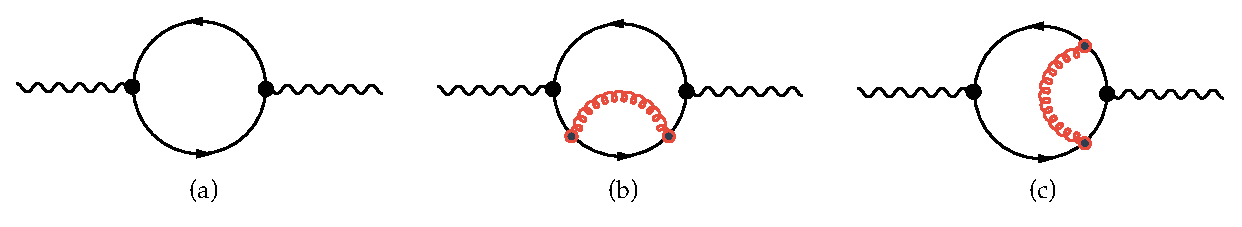
\includegraphics[width=\textwidth]{./images/correlatorLoopDiagrams.eps}
  \label{fig:perturbativeContributionFeynmanDiagrams}
\end{figure}
\begin{equation}
  \left. \Pi^B_{\mu\nu}(q^2) \right\rvert^{1-loop} = \frac{N_c}{12\pi^2} \left( \frac{1}{\hat \epsilon} - \log\frac{(-q^2 - i0)}{\mu^2} + \frac{5}{3} + \mathcal{O}(\epsilon) \right),
\end{equation}
where \(\Pi^B_{\mu\nu}(q^2)\) is the bare two\-/point function and is not
renormalised\footnote{The term \(1/ \hat \epsilon\), which is of order zero in
  \(\alpha_s\), will be cancelled by renormalisation.} This result can then be
used to extract the first two coefficients of the correlator expansion given in
\cref{eq:correlatorExpansion}
\begin{equation}
  c_{00} = - \frac{5}{3} \qquad \text{and} \qquad c_{01} = 1.
\end{equation}

The second loop can also be calculated by diagram techniques resulting in
\cite{Boito2011}
\begin{equation}
  \left. \Pi_V^{(1+0)}(s) \right\rvert^{2-loop} = -\frac{N_c}{12\pi^2} a_\mu \log(\frac{-s}{\mu^2}) + \cdots
\end{equation}
yielding $c_{11} = 1$.

Beginning from three loop diagrams the algebra becomes exhausting and one has to
use dedicated algorithms to compute the higher loops. The third loop
calculations have been done in the late seventies by
\cite{Chetyrkin1979,Dine1979,Celmaster1979}. The four loop evaluation have been
completed a little more than ten years later by
\cite{Gorishnii1990,Surguladze1990}. The highest loop published, that amounts to
$\alpha_s^4$, was published in 2008 \cite{Baikov2008} almost 20 years later.

Fixing the number of colors to $N_c=3$ the missing coefficients up to order four
in $\alpha_s$ read:
\begin{equation}
  \label{eq:adlerCoefficients}
  \begin{split}
    c_{2,1} &= \frac{365}{24} - 11 \zeta_3 - \left( \frac{11}{12} - \frac{2}{3}\zeta_3 \right) N_f \\
    c_{3,1} &= \frac{87029}{288} - \frac{1103}{4} \zeta_3 + \frac{275}{6}\zeta_5 \\
    &- \left( \frac{7847}{216} - \frac{262}{9} \zeta_3 + \frac{25}{9} \zeta_5 \right) N_f + \left( \frac{151}{162} - \frac{19}{27}\zeta_3\right)N_f^2 \\
    c_{4,1} &= \frac{78631453}{20736} - \frac{1704247}{432}\zeta_3 +
    \frac{4185}{8}\zeta_3^2 + \frac{34165}{96}\zeta_5 - \frac{1995}{16}\zeta_7,
  \end{split}
\end{equation}
where used the flavor number $N_f=3$ for the last line.

The 6-loop calculation has until today not been achieved, but Beneke and Jamin
\cite{Beneke2008} used and educated guess to estimate the coefficient
\begin{equation}
  c_{5,1} \approx 283 \pm 283.
\end{equation}

In stating the coefficients \(c_{n,k}\) of the correlator expansion we have
restricted ourselves to \(k\)\-/indices equal to one. This is due to the
\textsc{rge}, which relates coefficients with \(k\) different than one to the
already stated coefficients \(c_{n,1}\). To relate the coefficients we have to
make use of the \textsc{rge}. Consequently the correlator \(\Pi_V^{T+L}(s)\)
needs to be a physical quantity, which we can be achieved with the previously
defined Adler function (\cref{eq:adlerFunction}). The correct expression for the
correlator expansion in \cref{eq:correlatorExpansion} is then given by
\begin{tcolorbox}[ams equation,myformula]
  D_V^{(1+0)} = - s \od{\Pi_V^{(1+0)}(s)}{s} = \frac{N_c}{12 \pi^2}
  \sum_{n=0}^\infty a_\mu^n \sum_{k=1}^{n+1} k c_{n,k} L^{k-1},
\end{tcolorbox}
where we used \(\dif L^k/ \dif s=k\ln(-s/\mu^2)^{k-1}(-1/\mu^2)\). Applying the
\textsc{rge} (\cref{eq:rge}) to the scale\-/invariant Adler function yields
\begin{equation}
  \label{eq:rgeAdler}
  -\mu \od{}{\mu} D_V^{(1+0)} = -\mu \od{}{\mu} \left( \pd{}{L} \dif L + \pd{}{a_s} \dif a_s \right) D_V^{1+0}
  = \left( 2\pd{}{L} + \beta \pd{}{a_s} \right) D_V^{1+0} = 0,
\end{equation}
where we made use of the \(\beta\) function, which is defined in
\cref{eq:betaFunction}, and of the expression \(\dif L / \dif \mu = - 2/ \mu\).

The relation between the correlator expansion coefficients can then be taken by
calculating the Adler function for a desired order and plugging it into the
\textsc{rge}. For example the Adler function to the second order in \(\alpha_s\)
\begin{equation}
  \label{eq:adler2ndOrder}
  D(s) = \frac{N_c}{12 \pi^2} \left[ c_{01} + a_\mu(c_{11} + 2 c_{12} L) + a_\mu^2(c_{21} + 2 c_{22} L + 3 c_{23} L^2) \right],
\end{equation}
can be inserted into \textsc{rgeAdler}
\begin{equation}
  4 a_\mu c_{12} + 2 a_\mu^2(2 c_{22} + 6 c_{23} L) + \beta_1 a_\mu^2(c_{11} + 2 c_{12}L) + \mathcal{O}(a_\mu^3) = 0
\end{equation}
to compare the coefficients order by order in \(\alpha_s\). At order
\(\alpha_\mu\) only the \(c_{12}\) term is present and has consequently to be
zero. For \(\mathcal{O}(a_\mu^2 L)\) only \(c_{23}\) exists as \(c_{12}=0\) and
thus also has to vanish. Finally at \(\mathcal{O}(a)\) we can relate \(c_{22}\)
with \(c_{11}\) resulting in:
\begin{equation}
  c_{12} = 0, \quad c_{22} = \frac{\beta_1 c_{11}}{4} \quad \text{and} \quad c_{23} = 0.
\end{equation}
Implementing the newly obtained Adler coefficients we can write out the Adler
function to the first order:
\begin{equation}
  D(s) = \frac{N_c}{12 \pi^2} \left[ c_{01} + c_{11} a_\mu \left( c_{21} - \frac{1}{2} \beta_1 c_{11} L  \right) a_\mu^2 \right] + \mathcal{O}(a_\mu^3).
\end{equation}

\textcolor{red}{continue here} We have used the \textsc{rge} to relate
Adler-function coefficients and thus reduce its numbers. But as we will see in
the following section the \textsc{rge} gives us two different choices in the
order of the computation of the perturbative contribution to the inclusive tau
decay ratio.

\subsubsection{Renormalization group summation}
By making use of the \textsc{rge} we have to decide about the order of
mathematical operations we perform. As the perturbative contribution
\(\delta_{pt}}\) is independent on the scale \(\mu\) we are confronted with two
choices \define{fopt}{fixed\-/order perturbation theory} or
\define{cipt}{contour\-/improved perturbation theory}. Each of them yields a
different result, which is the main source of error in extracting the strong
coupling from tau decays.

We can write the perturbative contribution \(\delta_{pt}\) of \(R_\tau\)
(\cref{eq:rTauContributions}) in the chiral limit, such that the longitudinal
contribution \(D^{(0)}\), in \cref{eq:rTauFinal} vanishes. Thus inserting the
expansion of \(D_V^{(1+0)}\) into the hadronic tau decay width
\cref{eq:rTauFinal} yields
\begin{equation}
  \label{eq:rTauDelta0}
  \delta_{pt} = \sum_{n=1}^{\infty} a_\mu^n \sum_{k=1}^n k c_{n,k} \frac{1}{2 \pi i} \oint_{\abs{x}=1} \frac{\dif x}{x} (1-x)^3(1+x) \log \left( \frac{-m_\tau^2 x}{\mu^2} \right)^{k-1}.
\end{equation}
Keep in mind that the contributions from the vector and axial-vector correlator
are identical in the massless case:
\begin{equation}
  D^{(1+0)} = D^{(1+0)}_V + D^{(1+0)}_A = 2 D^{(1+0)}_V.
\end{equation}

To continue evaluating the perturbative part we can now either follow the
description of \textsc{fopt} or \textsc{cipt}. We will now present both.

In \textsc{fopt} we fix the scale at the tau mass (\(\mu^2=m_\tau^2\)), which
leaves us with the integration over the logarithm, as seen in
\begin{equation}
  \delta_{FO}^{(0)} = \sum_{n=1}^\infty a(m_\tau^2)^n \sum_{k=1}^n k c_{n,k} J_{k-1}
\end{equation}
where the contour integrals \(J_l\) are defined by
\begin{equation}
  J_l \equiv \frac{1}{2\pi i} \oint_{\abs{x}=1} \frac{\dif x}{x} (1-x)^3(1+x) \log^l(-x).
\end{equation}
The integrals \(J_l\) up to order \(\alpha_s^4\) are given by \cite{Beneke2008}:
\begin{equation}
  J_0 = 1, \quad J_1 = -\frac{19}{12} \quad J_2 = \frac{265}{72} - \frac{1}{3} \pi^2, \quad J_3 = - \frac{3355}{288} + \frac{19}{12}\pi^2.
\end{equation}
Using \textsc{fopt} the strong coupling \(a(\mu)\) is fixed at the tau mass
scale \(a(m_\tau^2)\) and can be taken out of the closed-contour integral. Thus
we solely have to integrate over the logarithms \(\log(x)\).

Using \textsc{cipt} we can sum the logarithms by setting the scale to \(\mu^2 = -m_\tau^2
x\) in \cref{eq:rTauDelta0}, resulting in:
\begin{equation}
  \delta^{(0)}_{CI} = \sum_{n=1}^\infty c_{n,1} J_n^a(m_\tau^2),
\end{equation}
where the contour integrals $J_l$ are defined by
\begin{equation}
  J_n^a(m_\tau^2) \equiv \frac{1}{2 \pi i} \oint_{\abs{x}=1} \frac{\dif x}{x} (1-x)^3(1+x) a^n(-m_\tau^2 x).
\end{equation}
Note that all logarithms vanish, except the ones with index \(k=1\):
\begin{equation}
  \log(1)^{k-1} =  \begin{cases} \mbox{1} & \mbox{if } k=1, \\ \mbox{0} & k\neq 1 \end{cases}
\end{equation}
which selects the Adler function coefficients \(c_{n,1}\). Handling the
logarithms left us with the integration of \(\alpha_s(- m_\tau^2 x)\) over the
closed-contour \(\oint_{\abs{x}=1}\), which now depends on the integration
variable \(x\).

In general we have to decide if we want to perform a contour integration with a
constant coupling constant and variable logarithms (\textsc{fopt}) or ``constant
logarithms'' and a running coupling (\textsc{cipt}). To emphasize the
differences in both approaches we can calculate the perturbative contribution
\(\delta^{(0)}\) to \(R_\tau\) for the two different prescriptions yielding
\cite{Beneke2008}
\begin{align}
  & \quad\qquad \alpha_s^2 \qquad \alpha_s^2 \qquad \alpha_s^3 \qquad \alpha_s^4 \quad\qquad \alpha_s^5 \nonumber\\
  \delta_{FO}^{(0)} &= 0.1082 + 0.0609 + 0.0334 + 0.0174 (+ 0.0088) = 0.2200 (0.2288) \\
  \delta_{CI}^{(0)} &= 0.1479 + 0.0297 + 0.0122 + 0.0086 (+ 0.0038) = 0.1984 (0.2021).
\end{align}
The series indicate, that \textsc{cipt} converges faster and that both series
approach a different value. This discrepancy represents currently the biggest
theoretical uncertainty while extracting the strong coupling.

As today we do not know if \textsc{fopt} or \textsc{cipt} is the correct
approach of measuring the strong coupling. Therefore there are currently three
ways of stating results: Quoting the average of both results, quoting the
\textsc{cipt} result or quoting the \textsc{fopt} result. We follow the approach
of Beneke and Jamin \cite{Beneke2008} who prefere \textsc{fopt}, but also state
their results in \textsc{cipt}.


\subsection{The Non-Perturbative OPE Contribution}
The perturbative contribution to the sum rule is the dominant one. The
contribution of the \textsc{npt} part can be quoted as
\begin{equation}
  \delta_{NP} = 0,007 \pm 0.004 \qquad \cite{Braaten1991},
\end{equation}
which is small, but not negligible. The \textsc{np} \textsc{ope} contributions
are commonly categorised by even, increasing dimensions. Contributions of
dimension larger than eight are normally neglected, due to the increasing
suppression by factors of \(1/m_\tau^{2D}\), where \(D\) stands for the
corresponding dimension.

The dimension two contributions are proportional to the quark masses. As we are
working in the chiral limit we will neglect them.

\subsection{Dimension four}
The next apparent \textsc{ope} contribution is of dimension four. Here we have
to take into account the terms with masses to the fourth power $m^4$, the quark
condensate multiplied by a mass $m \langle \anti{q} q \rangle$ and the gluon
condensate $\langle GG \rangle$. The resulting expression can be taken from the
appendix of \cite{Pich1999}, yielding:
\begin{equation}
  \left. D_{ij}^{(1+0)}(s) \right\rvert_{D=4} = \frac{1}{s^2} \sum_n \Omega^{(1+0)}(s/\mu^2)a^n,
\end{equation}
where
\begin{equation}
  \begin{split}
    \Omega_n^{(1+0)} (s/\mu^2) &\,=\, \frac{1}{6}\langle aGG \rangle p_n^{(1+0)}(s/\mu^2) + \sum_k m_k \langle \anti{q}_k q_k \rangle r_n^{(1+0)}(s/\mu^2) \\
    &\,+ 2\langle m_i \anti{q}_i q_i + m_j \anti{q}_j q_j \rangle q_n^{(1+0)} (s/\mu^2) \pm \frac{8}{3} \langle m_j \anti{q}_i q_i + m_i \anti{q}_j q_j \rangle t_n^{(1+0)} \\
    &\,- \frac{3}{\pi^2} (m_i^4 + m_j^4) h_n^{(1+0)} (s/\mu^2) \mp \frac{5}{\pi^2} m_i m_j (m_i^2 + m_j^2) k_n^{(1+0)}(s/\mu^2)\\
    &\,+ \frac{3}{\pi^2} m_i^2 m_j^2 g_n^{(1+0)}(s/\mu^2) + \sum_k m_k^4
    j_n^{(1+0)}(s/\mu^2) + 2 \sum_{k \neq l} m_k^2 m_l^2 u_n^{(1+0)}(s/\mu^2)
  \end{split}
\end{equation}
The perturbative expansion coefficients are known to $\mathcal{O}(a^2)$ for the
condensate contributions,
\begin{equation}
  \begin{array}{lll}
    p_0^{(1+0)}=0, & p_1^{(1+0)}=1, & p_2^{(1+0)}=\frac{7}{6}, \\
    r_0^{(1+0)}=0, & r_1^{(1+0)}=0, & r_2^{(1+0)}=-\frac{5}{3}+\frac{8}{3}\zeta_3-\frac{2}{3}\log(s/\mu^2), \\
    q_0^{(1+0)}=1, & q_1^{(1+0)}=-1, & q_2^{(1+0)}=-\frac{131}{24}+\frac{9}{4}\log(s/\mu^2) \\
    t_0^{(1+0)}=0 & t_1^{(1+0)}=1, & t_2^{(1+0)}=\frac{17}{2}+\frac{9}{2}\log(s/\mu^2).
  \end{array}
\end{equation}
while the $m^4$ terms have been only computed to $\mathcal{O}(a)$
\begin{equation}
  \begin{array}{lll}
    h_0^{(1+0)}=1-1/2 \log(s/\mu^2), & h_1^{(1+0)}=\frac{25}{4}-2\zeta_3-\frac{25}{6}\log(s/\mu^2)-2 \log(s/\mu^2)^2, \\
    k_0^{(1+0)}=0, & k_1^{(1+0)}=1-\frac{2}{5}\log(s/\mu^2), \\
    g_0^{(1+0)}=1, & g_1^{(1+0)}=\frac{94}{9}-\frac{4}{3}\zeta_3-4 \log(s/\mu^2), \\
    j_0^{(1+0)}=0, & j_1^{(1+0)}=0, \\
    u_0^{(1+0)}=0, & u_2^{(1+0)}=0.
  \end{array}
\end{equation}

\subsection{Dimension six and eight}
Our application of dimension six contributions is founded in \cite{Braaten1991}
and has previously been calculated beyond leading order by \cite{Lanin1986}. The
operators appearing are the masses to the power six $m^6$, the four-quark
condensates $\langle \anti q q \anti q q \rangle$, the three-gluon condensates
$\langle g^3 G^3 \rangle$ and lower dimensional condensates multiplies by the
corresponding masses, such that in total the mass dimension of the operator will
be six. As there are too many parameters to be fitted with experimental data we
have to omit some of them, starting with the three-gluon condensate, which does
not contribute at leading order. The four-quark condensates known up to
$\mathcal{O}(a^2)$, but we will make use of the \textit{vacuum saturation
  approach} \cite{Beneke2008,Braaten1991,Shifman1978} to express them in quark,
anti-quark condensates $\langle q \anti{q} \rangle$. In our work we take the
simplest approach possible: Introducing an effective dimension six coefficient
$\rho_{V/A}^{(6)}$ divided by the appropriate power in s
\begin{equation}
  \left. D_{ij,V/A}^{(1+0)} \right\rvert_{D=6} = 0.03 \frac{\rho_{V/A}^{(6)}}{s^3}
\end{equation}

As for the dimension eight contribution the situation is not better than the
dimension six one we keep the simplest approach, leading to
\begin{equation}
  \left. D_{ij,V/A}^{(1+0)} \right\rvert_{D=8} = 0.04 \frac{\rho_{V/A}^{(8)}}{s^4}.
\end{equation}


\section{Duality Violations}
As seen in \cref{sec:duality} we have to assume quark\-/hadron duality for the
\textsc{qcdsr} to work. Unfortunately duality cannot always be taken for granted
and the existence of \define{dv}{duality violations} is a well known
\cite{Cata2008,Cata2009}. As we will see in the following section, the
experimental measured total tau decay ratio has a exponential decreasing,
sinusoidal contributions, that cannot be reproduced by the \textsc{ope} solely.
Consequently for the cases with apparent \textsc{dv} we also have to take into
account \textsc{dv} corrections and adapt \cref{eq:rTauContributions}
\begin{equation}
  R_{\tau,V/A}^\omega = \frac{N_c}{2}S_{EW} \abs{V_{ud}}^2 \left( 1 + \delta_{pt}^{\omega} + \delta_{npt}^{\omega} + \delta_{dv}^{\omega} \right).
\end{equation}
The \textsc{dv} correction has been modelled by a series of papers
\cite{Boito2011a,Boito2012,Boito2014} with the following ansatz 
\begin{equation}
  \rho_{V/A}^{DV}(s) = e^{-(\delta_{V/A}+\gamma_{V/A}s)} \sin(\alpha_{V/A} + \beta_{V/A}s),
\end{equation}
to parametrise the \textsc{dv} contributions. The \textsc{dv} would then appear
as an additional term in the inclusive tau decay ratio
\begin{equation}
  R_{\tau,V/A} = - \pi i \oint_{\abs{s}=m_\tau^2} \frac{\dif x}{x} (1 - x)^3 \left[ 3
    (1 + x) D^{(1+0)}(m_\tau^2 x) + 4 D^{(0)}(m_\tau^2 x) \right] +  \mathcal{D}_{V/A}(m_\tau^2),
\end{equation}
where the \textsc{dv} would be given as
\begin{equation}
  \mathcal{D}_\omega(m_\tau^2) = -12 \pi^2 \int_{m_\tau^2}^\infty \frac{\dif s}{m_\tau^2} \omega(s) \rho_{V/A}.
\end{equation}

\subsection{Pinched weights to avoid DVs}
We are free to multiply \cref{eq:correlatorContourIntegral} by an analytic
weight function $\omega(s)$
\begin{equation}
  \int_0^{m_\tau} \omega(s) \Pi(s) \dif s = \frac{i}{2} \oint_{s=m_\tau} \omega(s) \Pi(s) \dif s.
\end{equation}
We can use this technique to suppress contributions for the two-point function
close to the positive real axis by implementing so called pinched weights of the
form
\begin{equation}
  \omega(s) = \left(1-\frac{s}{m_\tau^2}\right)^k,
\end{equation}
where k is the degree of the pinched weight. The higher the degree the farther
we operate from the critical positive real axis (see.
\cref{fig:pinchedWeightGraphs}), which suppresses the effects of duality
violations. This pinching of second degree appears quite naturally.
\begin{figure}
  \centering
  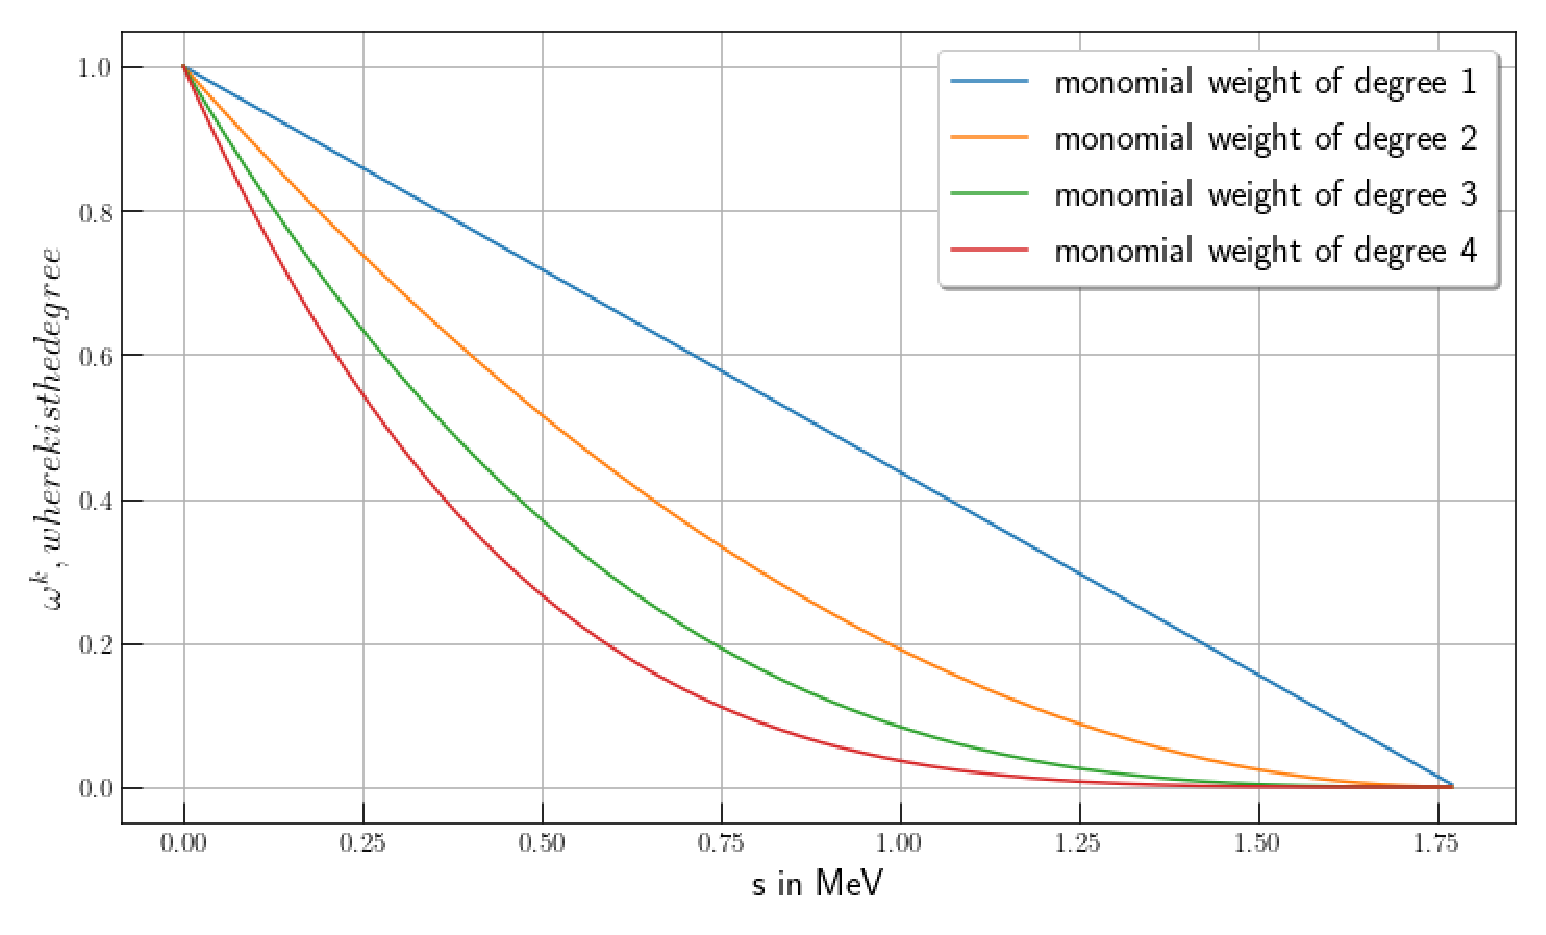
\includegraphics[width=\textwidth]{./images/monomialWeightGraphs.eps}
  \caption{Monomial weights $(1-s/m_\tau^2)^k$ for degrees $1\to4$. We can see
    that weights of higher pinching decrease faster, which comes in handy if we
    want to suppress duality violations.}
  \label{fig:monomialWeightGraphs}
\end{figure}
If we regard the include $\tau-decay$ ratio \cref{eq:rTauT+L}, we note that for
the transversal component we already have a double pinched weight, the
\textit{kinematic weight}
\begin{equation}
  \label{eq:kinematicWeight}
  \omega_\tau(s) = \left( 1-\frac{s}{m_\tau^2} \right)^2 \left( 1 + 2 \frac{s}{m_\tau^2} \right).
\end{equation}
In general it is said that a double pinched weight is sufficient to neglect
effects caused by duality violation.



\section{Experiment}
The $\tau$-decay data we use to perform our QCD-analysis is from the
\textbf{ALEPH} experiment. The ALEPH experiment was located at the
large-electron-positron (LEP) collider at CERN laboratory in Geneva. LEP started
producing particles in 1989 and was replaced in the late 90s by the
large-hadron-collider, which makes use of the same tunnel of 27km circumference.
The data produced within the experiment is still maintained by former ALEPH
group members under led by M. Davier, which have performed regular updates on
the data-sets \cite{Davier2013,Davier2008,Aleph2005}.

The measured spectral functions for the Aleph data are defined in
\cite{Davier2007} and given for the transverse and longitudinal components separately:
\begin{equation}
  \begin{split}
    \rho^{(T)}_{V/A}(s) &= \frac{m_\tau^2}{12 \abs{V_{ud}^2}S_{EW}} \frac{\mathcal{B}(\tau^- \to V^-/A^- \nu_\tau)}{\mathcal{B}(\tau^- \to e^- \anti{\nu}_e \nu_\tau)} \\
    &\quad\times \frac{\dif N_{V/A}}{N_{V/A}\dif s} \left[ \left( 1 - \frac{s}{m_\tau^2} \right)^2 \left( 1 + \frac{2s}{m_\tau^2} \right) \right]^{-1} \\
  \rho^{(L)}_{A}(s) &= \frac{m_\tau^2}{12 \abs{V_{ud}^2 S_{EW}}} \frac{\mathcal{B}(\tau^- \to \pi^-(K^-) \nu_\tau)}{\mathcal{B}(\tau^- \to e^- \anti{\nu}_e \nu_\tau)} \times \frac{\dif N_A}{N_A \dif s} \left( 1 - \frac{s}{m_\tau^2} \right)^{-2}.
  \end{split}
\end{equation}

\begin{equation}
  \mathcal{B}_e = ...
\end{equation}

\begin{equation}
  R_{\tau, V/A} = \frac{B_{V/A, \tau}}{B_e}
\end{equation}

The data relies on a separation into vector and axial-vector channels. In the
case of the Pions this can be achieved via counting. The vector channel is
characterised by a negative parity, whereas the axial-vector channel has
positive parity. A quark has by definition positive parity, thus an anti-quark
has a negative parity. A meson, like the Pion particle, is a composite particle
consisting of an quark an anti-quark. Consequently a single Pion carries negative
parity, an even number of Pions carries positive parity and an odd number of
Pions carries negative parity:
\begin{equation}
  n \times \pi = \begin{cases} \mbox{vector} & \mbox{if } n \text{ is even}, \\ \mbox{axial-vector} & \mbox{otherwise} \end{cases}.
\end{equation}

The contributions to the vector and axial channel can be seen in
\textcolor{red}{figure}. The dominant modes in the vector case are
\cite{Davier2006} $\tau^- \to \pi^-\pi^0 \nu_\tau$ and the $\tau^- \to \pi^-
\pi^- \pi^+ \pi^0 \nu_\tau$. The first of these is produced by the $\rho(770)$
meson, which in contrary to the pions carries angular momentum of one, which is
also clearly visible as peak around $\SI{770}{\giga\eV}$ in
\textcolor{red}{figure vector}. The dominant modes in the axial-vector case are
$\tau^-\to \pi^-\nu_\tau$, $\tau^-\to \pi^- \pi^0 \pi^0 \nu_\tau$ and
$\tau^- \to \pi^- \pi^- \pi^+\nu_\tau$. Here the three pion final states stem
from the $a_1^-$-meson, which is also clearly visible as a peak in \textcolor{red}{figure}.
\begin{figure}
    \centering
    \begin{subfigure}[b]{0.49\textwidth}
        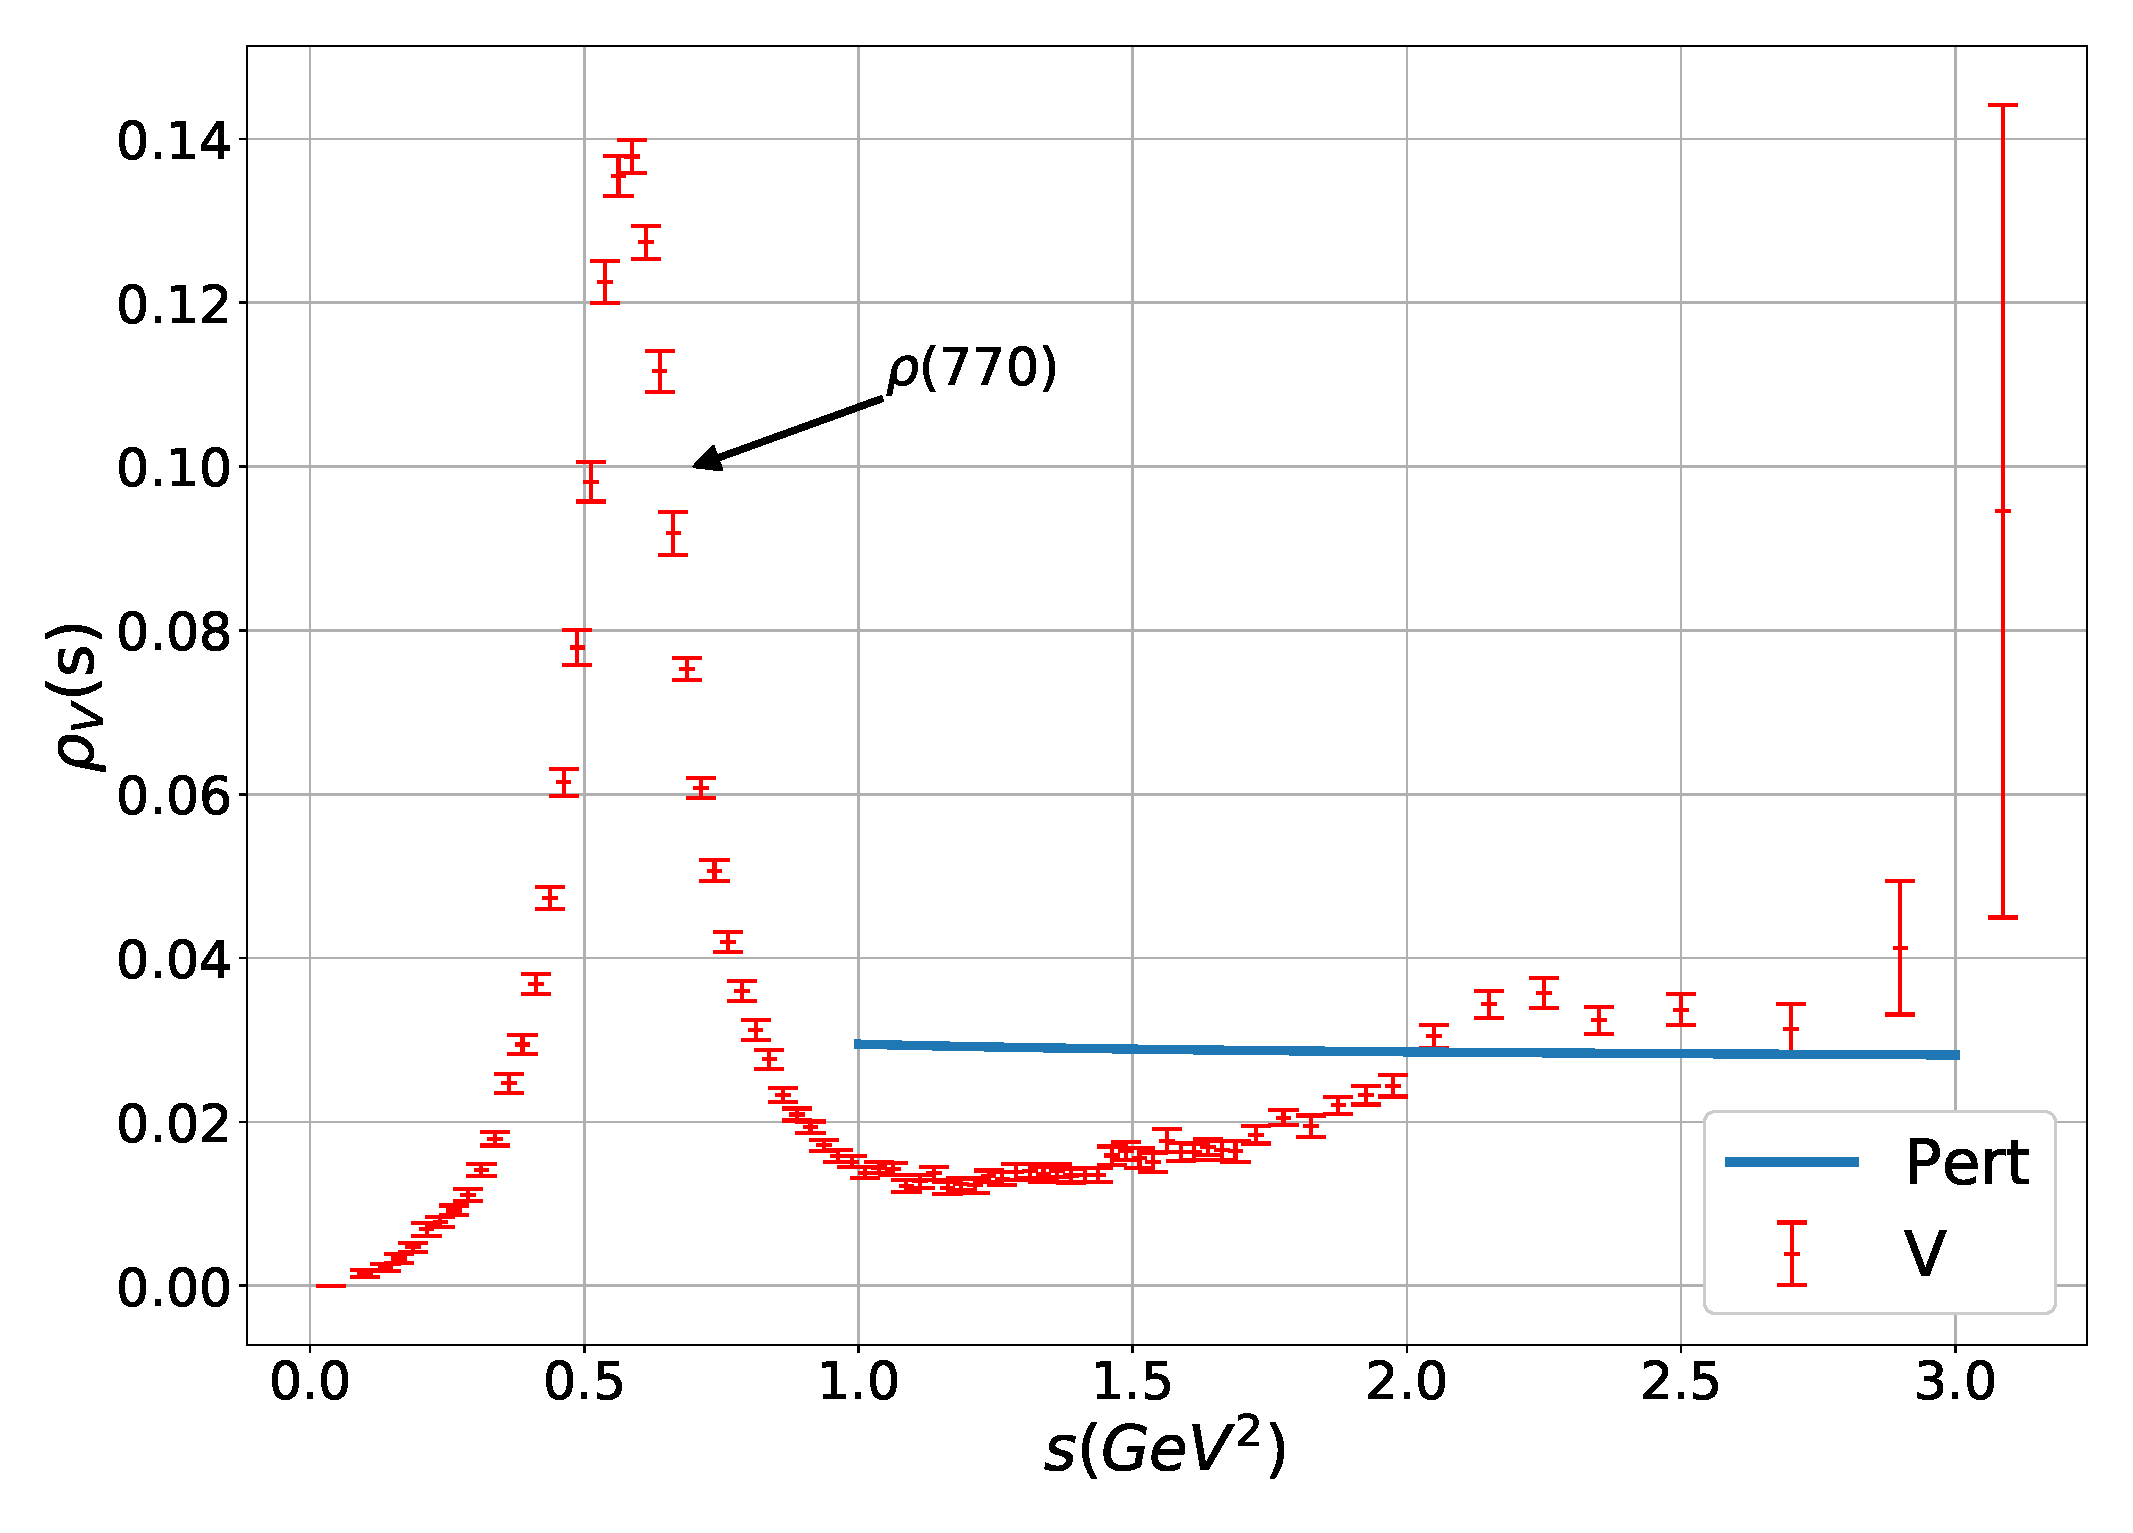
\includegraphics[width=\textwidth]{./images/specFuncAleph_V.eps}
        \caption{A gull}
        \label{fig:gull}
    \end{subfigure}
    \begin{subfigure}[b]{0.49\textwidth}
        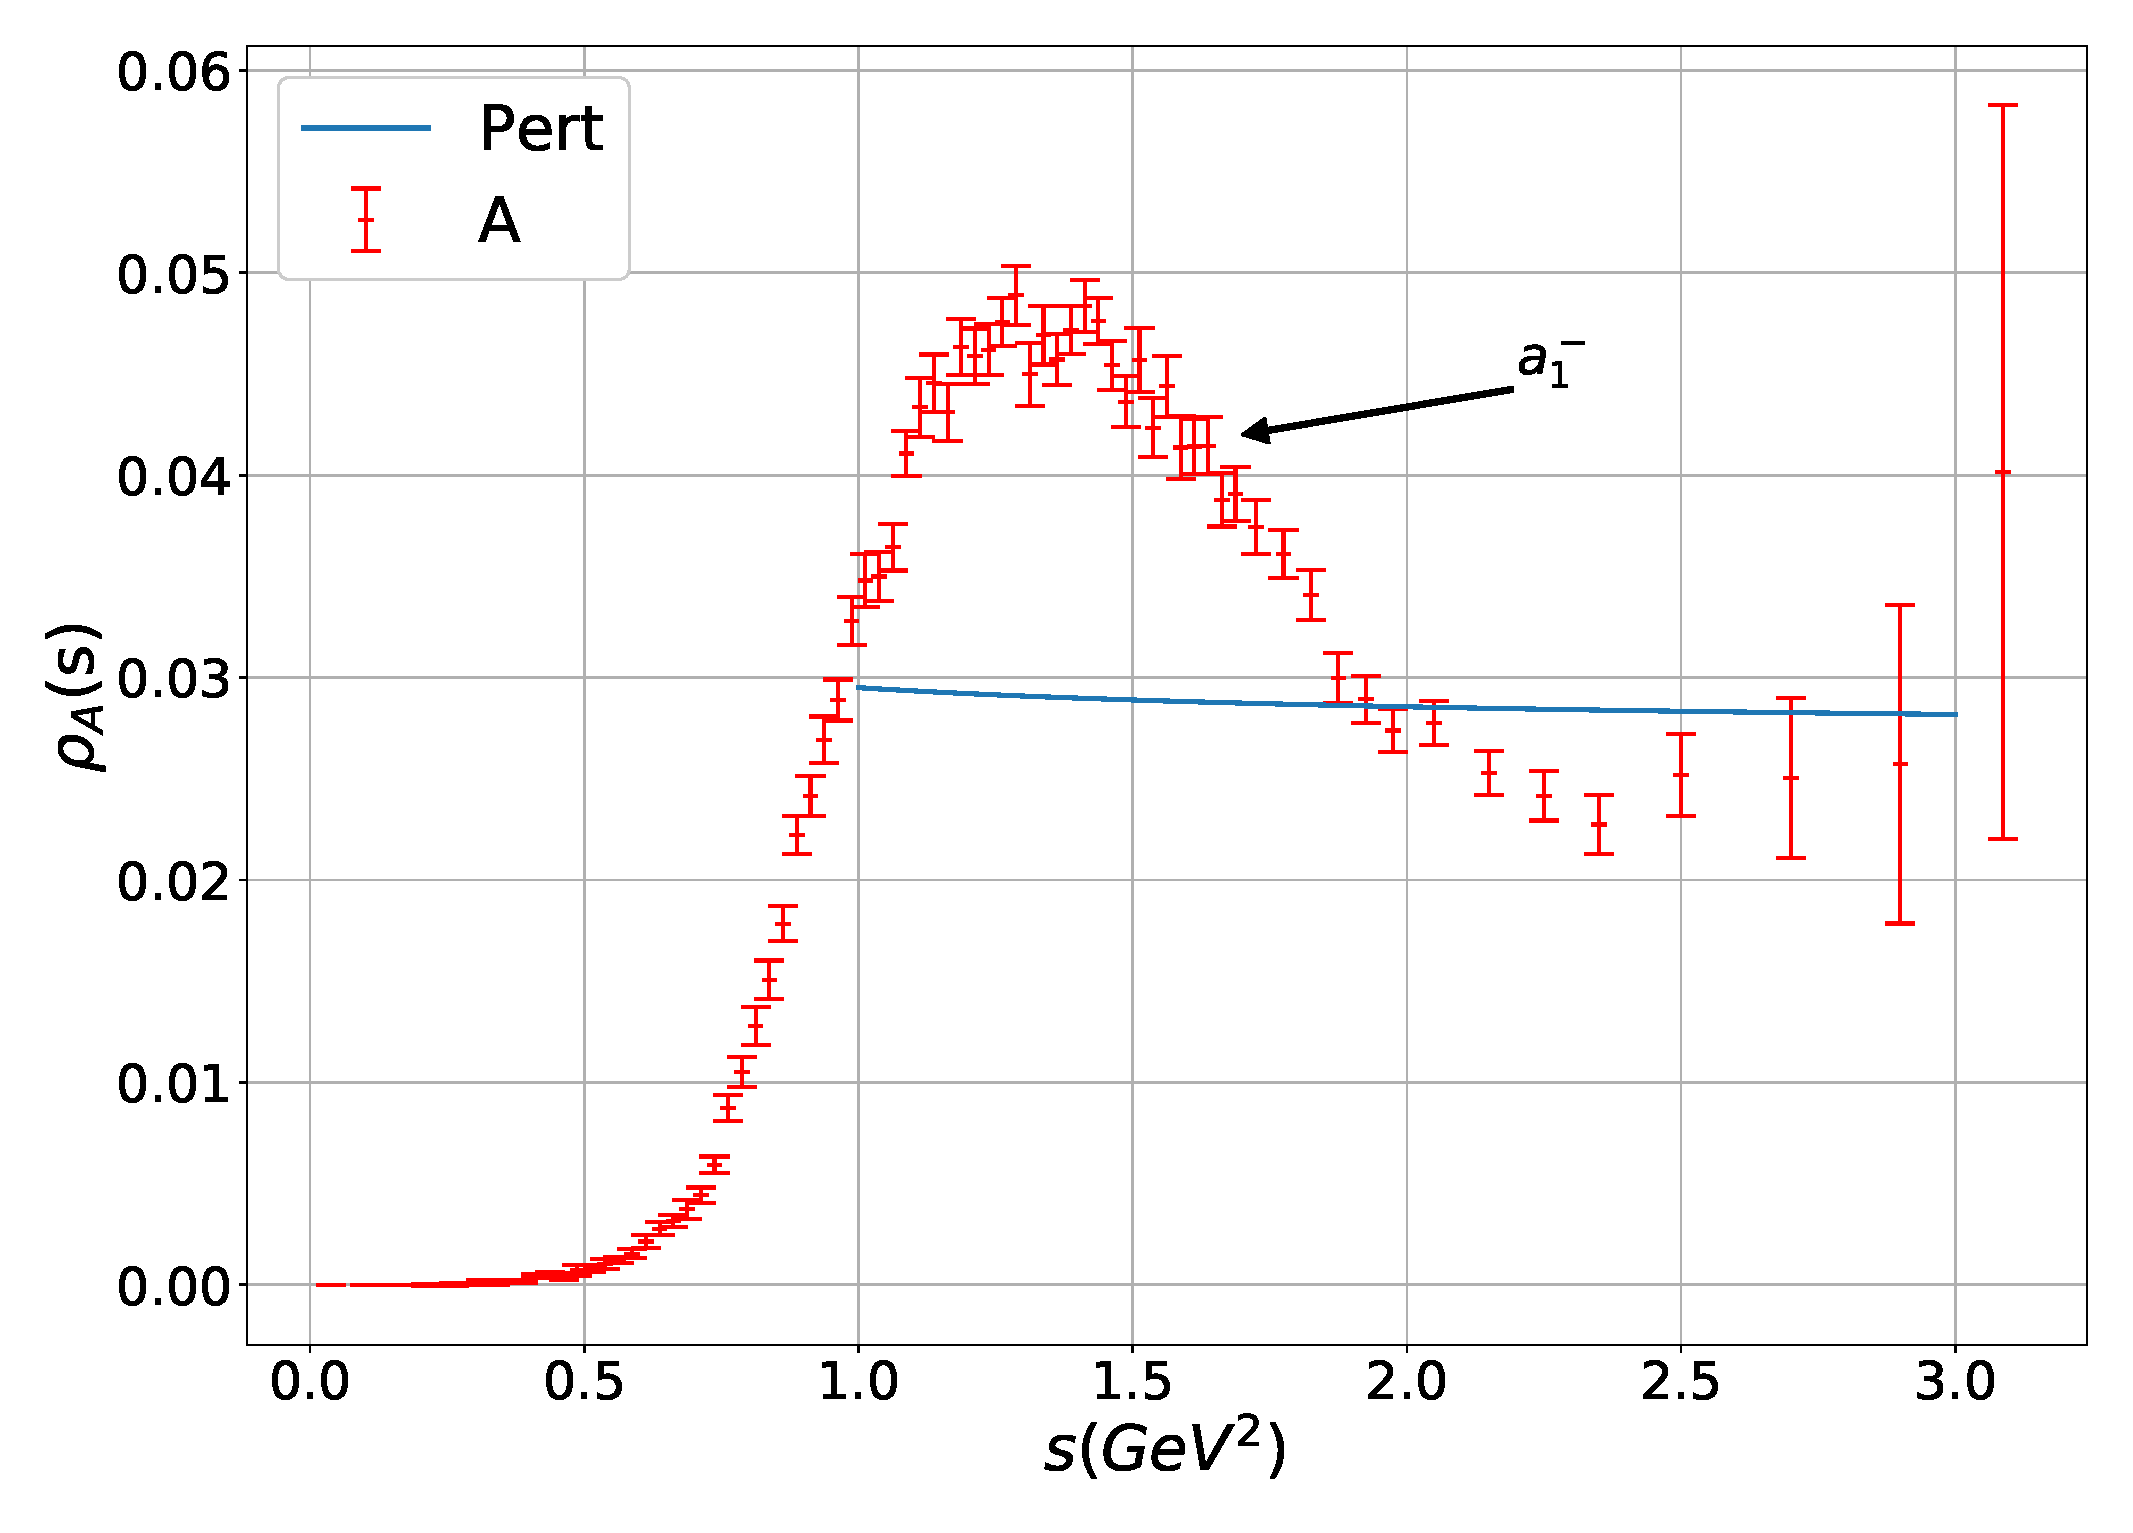
\includegraphics[width=\textwidth]{./images/specFuncAleph_A.eps}
        \caption{A mouse}
        \label{fig:mouse}
    \end{subfigure}
    \begin{subfigure}[b]{0.8\textwidth}
      \centering
      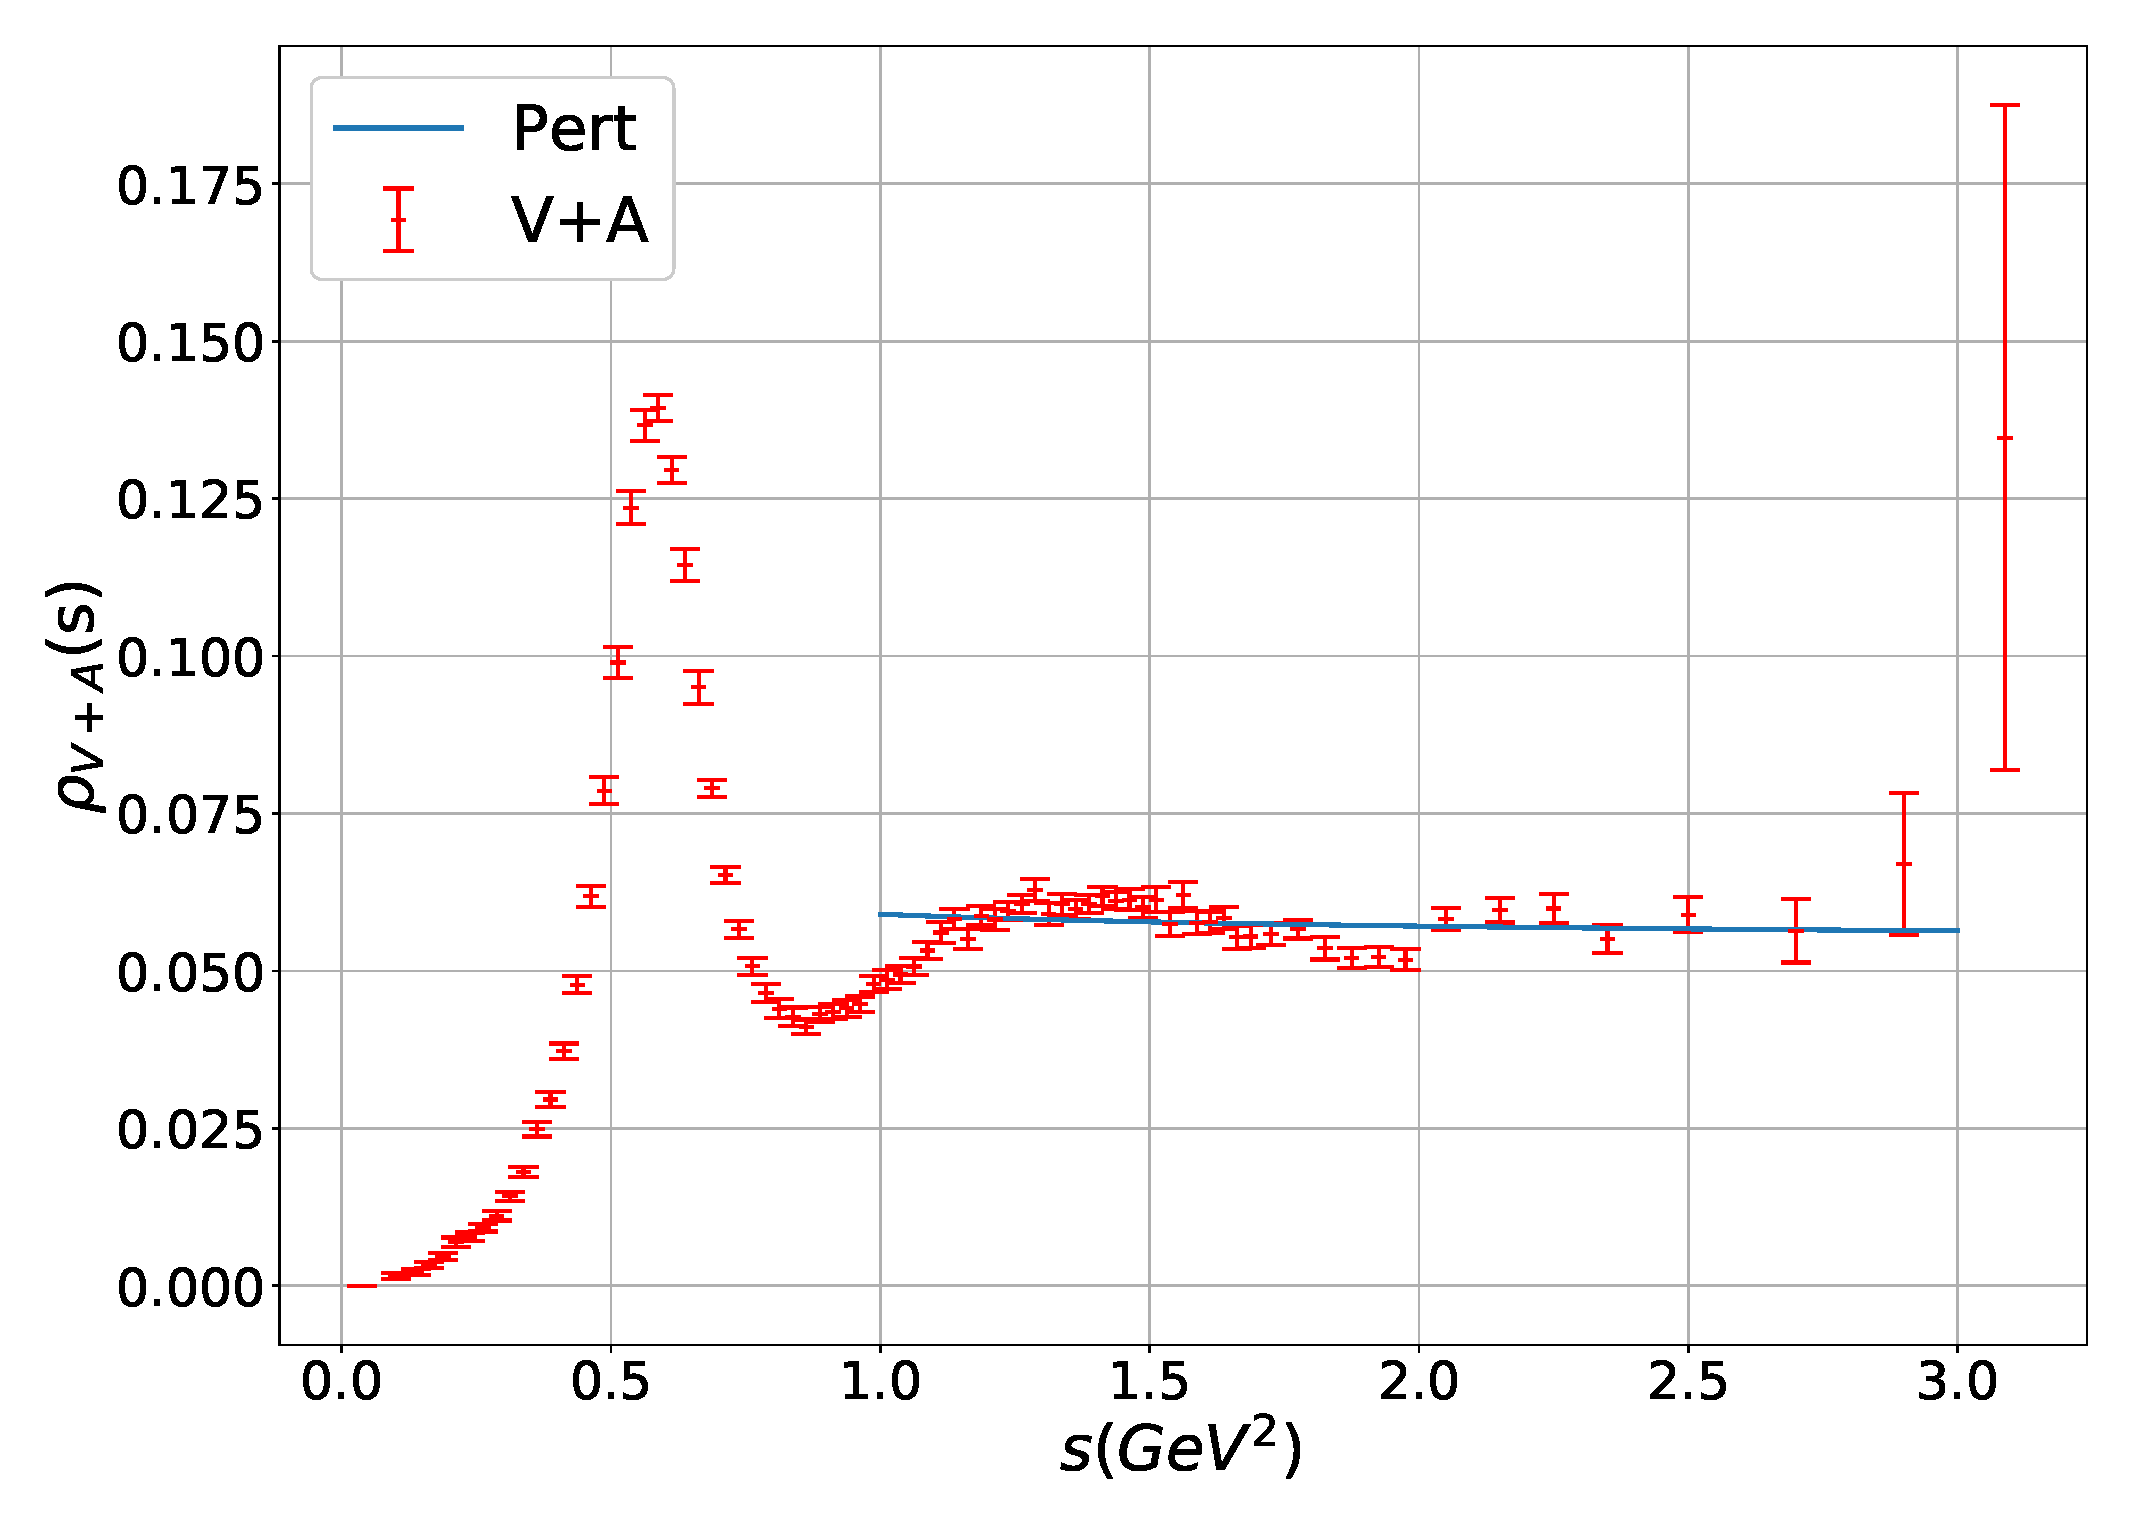
\includegraphics[width=\textwidth]{./images/specFuncAleph_VpA.eps}
      \label{fig:}
    \end{subfigure}
    \caption{Pictures of animals}\label{fig:animals}
\end{figure}

wavy => DV
OPE cannot reproduce
suppressed in VpA
regions below 1.5 GeV can still not be applied

The different inclusive $\tau$-decay ratios are then given by
\begin{align}
  R_{\tau,V} &= ...
\end{align}

\end{document}
% LocalWords:  adlerFunction rTauContributions adlerSndOrder betaFunction rTauT
% LocalWords:  correlatorExpansion correlatorLoopDiagrams antiderivatives AlD
% LocalWords:  longitudinalCorrelator monomialDimensions monomialInclusiveRatio
% LocalWords:  monomialWeights monomialWeightGraphs pinchedWeightGraphs llllll
% LocalWords:  hadronicTauDecayRatio correlatorContourIntegral LocalWords lllll
% LocalWords:  correlatorCombination fitWKinAlD rTauCauchysTheorem SpecFunc
% LocalWords:  cauchysTheorem fitWKinD twoPointFunction fitWCubicAlD fitWM
% LocalWords:  fitWCubeAlpha fitWCubeAlD wKinResults cubicWeight quarticWeight
% LocalWords:  correlatorTransversalLongitudinalDecomposition wFitM lllllll
% LocalWords:  inclusiveRatio theoreticalBackground
